% =====================================================================
%  GMN2 附录 E  二阶离散导数非正的整数组态（Configurations of integers with
%  nonpositive second discrete derivative）
%  原文：wkb-paper.tex 9873–9906 行；印刷页 p.174–175；编号公式 (E.1)–(E.2) 共 2 条
%  脚注 0 条；插图 3 幅：convexk-1（图 88）+ convexk-2（图 89）+ convexk-3（图 90）
%        原文是一处 \insthreefigs 并排、三个 \caption，故占三个图号；preamble 未定义该宏，
%        此处按 ch13/appA 先例展开为一个 figure + 三个 minipage，保留原三个图号
%  main.tex 第 67 行 \appendix 生效时，本节自动编号为 E，公式随之为 (E.1)…，与原文一致
%  块内引用（\eqref{eq:NegBetas2}）直接用；跨块引用（第 3.2 节、(3.42)）硬编码原文编号并加 % TODO
% =====================================================================

\section{二阶离散导数非正的整数组态}\label{app:ConvexKay}

这里我们总结一些关于整数族 $\{ k_\alpha \}$（$0 \leq \alpha \leq n+1$）的简单观察；这些整数出现在第 3.2 节% TODO 合稿改 \ref{subsec:WittenConstruction}
的 D4/NS5-膜位形中。按照 (3.42)，这些位形满足% TODO 合稿改 \eqref{eq:NegBetas}
\begin{equation} \label{eq:NegBetas2}
- 2k_\alpha + k_{\alpha+1} + k_{\alpha-1} + d_\alpha \leq 0, \qquad\qquad 1\leq \alpha \leq n.
\end{equation}
由于 $d_\alpha \geq 0$，\eqref{eq:NegBetas2} 表明：若把 $k_\alpha$ 看作 $\alpha$ 的函数，则它的二阶离散导数非正，即其图像是凸的。

\begin{figure}[htbp]
\centering
\begin{minipage}[b]{0.31\linewidth}
\centering 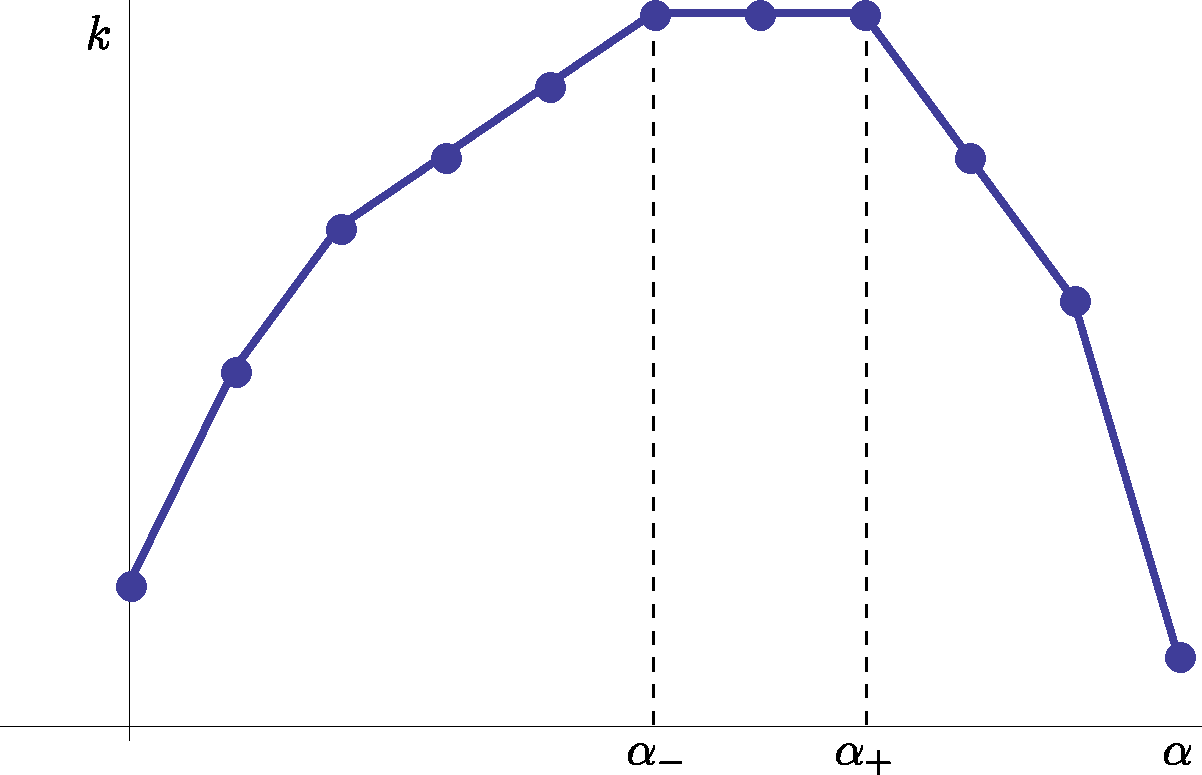
\includegraphics[width=1.15in]{figures/convexk-1-crop.pdf}
\caption{当 $k_1-k_0>0$ 时，满足 $2k_\alpha-k_{\alpha-1} - k_{\alpha+1}\geq 0$ 的一组整数 $k_\alpha$ 的典型图像。}\label{fig:convexk-1}
\end{minipage}\hspace{0.25cm}
\begin{minipage}[b]{0.31\linewidth}
\centering 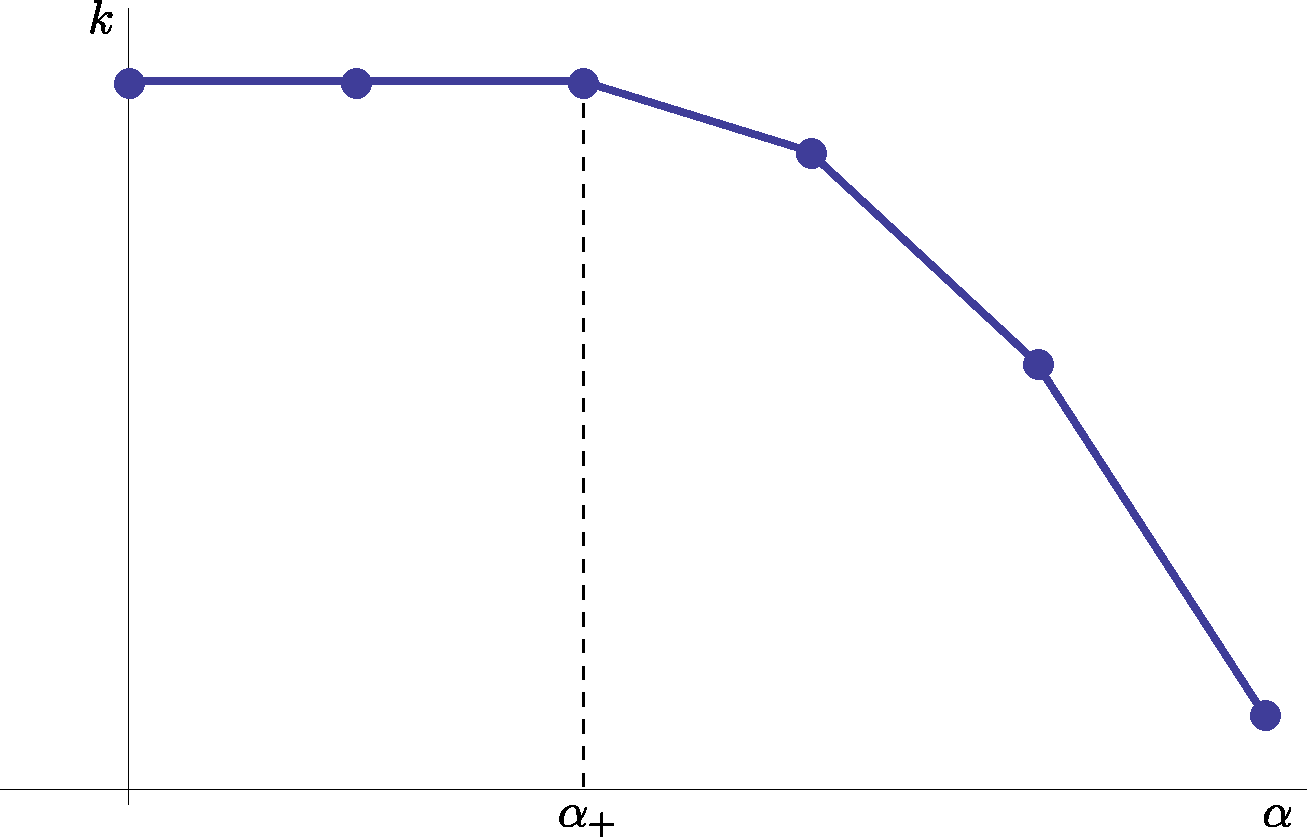
\includegraphics[width=1.15in]{figures/convexk-2-crop.pdf}
\caption{当 $k_1-k_0=0$ 时，满足 $2k_\alpha-k_{\alpha-1} - k_{\alpha+1}\geq 0$ 的一组整数 $k_\alpha$ 的典型图像。}\label{fig:convexk-2}
\end{minipage}\hspace{0.25cm}
\begin{minipage}[b]{0.31\linewidth}
\centering 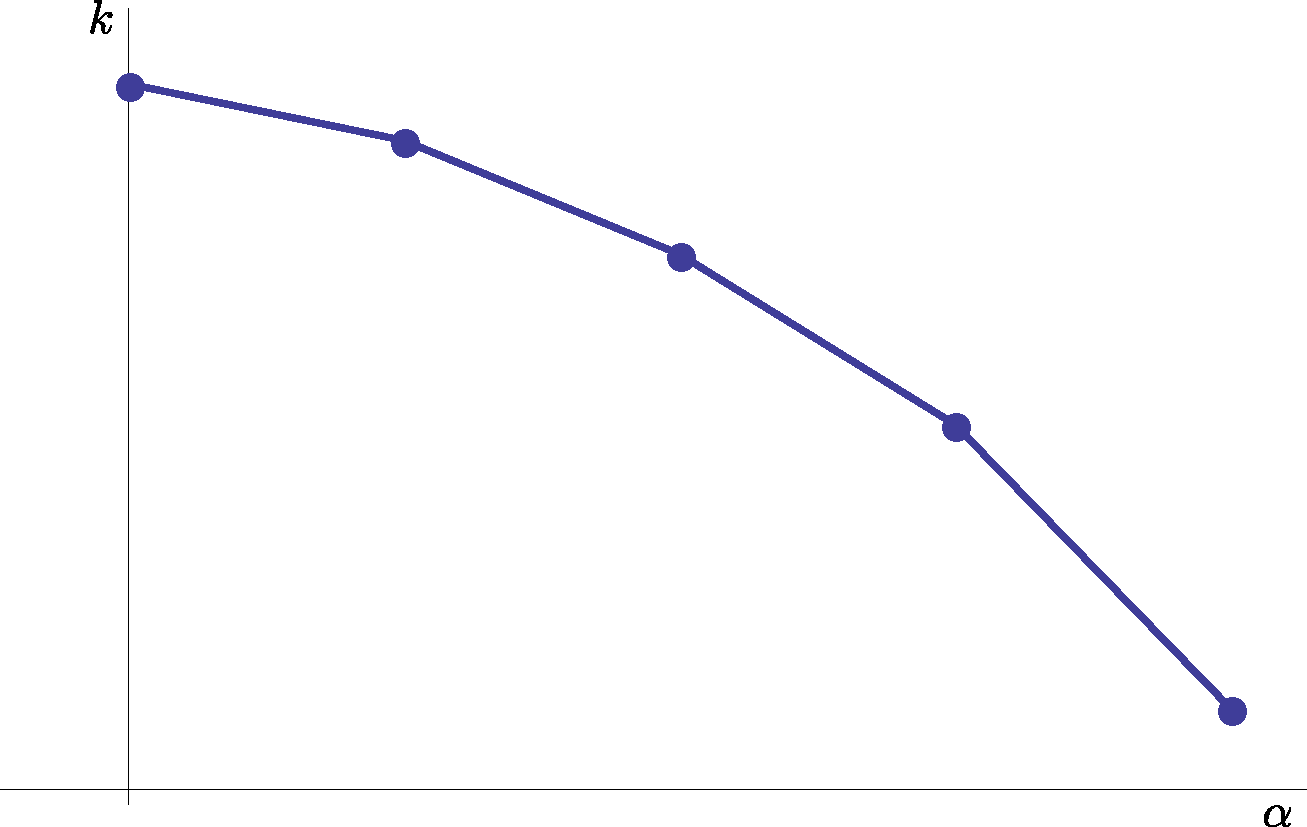
\includegraphics[width=1.15in]{figures/convexk-3-crop.pdf}
\caption{当 $k_1-k_0<0$ 时，满足 $2k_\alpha-k_{\alpha-1} - k_{\alpha+1}\geq 0$ 的一组整数 $k_\alpha$ 的典型图像。}\label{fig:convexk-3}
\end{minipage}
\end{figure}

要区分三种基本情形。第一种是 $k_1-k_0 > 0$。此时 $k_\alpha$ 在 $0\leq \alpha \leq \alpha_-$ 上严格递增，在 $\alpha_-\leq \alpha \leq \alpha_+$ 上取到最大值 $K$，并在 $\alpha \geq \alpha_+$ 上严格递减（见图 88）。% TODO 合稿改 \ref{fig:convexk-1}
若 $k_1 - k_0 = 0$，则行为类似，只是 $\alpha_- = 0$（见图 89）。% TODO 合稿改 \ref{fig:convexk-2}
最后，若 $k_1 - k_0 < 0$，则 $\alpha_- = \alpha_+ = 0$，如图 90 所示。% TODO 合稿改 \ref{fig:convexk-3}

还有一个重要的特殊情形：二阶离散导数恒为零，即对 $1 \leq \alpha \leq n$ 有 $-2k_\alpha + k_{\alpha+1} + k_{\alpha-1} = 0$。此时图像就是一条直线，亦即
\begin{equation}
k_\alpha = k_0 + \alpha r, \qquad\qquad 0 \leq \alpha \leq n+1.
\end{equation}
